\documentclass{llncs}
\usepackage{graphics}
\usepackage[dvips]{epsfig}
\usepackage[latin1]{inputenc}
\usepackage{color}
\usepackage{longtable}
\usepackage{multirow}
\usepackage[dvips]{graphicx} 
%\usepackage{amsmath}
\usepackage{textcomp}
\usepackage{url}

\newcommand{\tab}{\hspace{20mm}}

\setlength{\textfloatsep}{8pt plus 2pt minus 2pt}
\setlength{\intextsep}{8pt plus 2pt minus 2pt}

%#\def\BibTeX{{\rm B\kern-.05em{\sc i\kern-.025em b}\kern-.08em
%#    T\kern-.1667em\lower.7ex\hbox{E}\kern-.125emX}}

%\hyphenation{}


\begin{document}

%%%%%%%%%%%%%%%%%%%%%%%%%%%%%%%   TITLE   %%%%%%%%%%%%%%%%%%%%%%%%%%%%%%%

\title{Modelling Human Expert Behaviour in an Unreal Tournament\texttrademark~2004 Bot}
%\thanks{\footnotesize{This paper has been funded in part by project TIN2011-28627-C04-02 and project P08-TIC-03903 awarded by the Andalusian Regional Government.}}}

\titlerunning{Modelling an UT2K4 Expert Bot}

%%%%%%%%%%%%%%%%%%%%%%%%%%%%%%%   AUTHORS   %%%%%%%%%%%%%%%%%%%%%%%%%%%%%%%

\author{A.M. Mora \and F. Aisa \and R. Caballero \and P. Garc�a-S�nchez \and \\ P.A. Castillo \and J.J. Merelo \and P. De las Cuevas}
\authorrunning{A.M. Mora et al.}

\institute{Departamento de Arquitectura y Tecnolog\'{\i}a de Computadores.\\
Universidad de Granada (Spain)\\
\email{\{amorag,pgarcia,pedro,jmerelo,paloma\}@geneura.ugr.es, francisco\_aisa@hotmail.com, rcabamo@gmail.com}
}

\maketitle

%
%%%%%%%%%%%%%%%%%%%%%%%%%%%%%%%   ABSTRACT   %%%%%%%%%%%%%%%%%%%%%%%%%%%%%%%
%
\begin{abstract}
This paper presents a deep description of the design of an autonomous agent (bot) for playing 1 vs. 1 dead match mode in the first person shooter
Unreal Tournament\texttrademark~2004 (UT2K4). 
The bot models most of the behaviour (actions and tricks) of an expert human player in this mode, who has participated in international UT2K4 championships.
The Artificial Intelligence engine is based on two levels of states, and it relies on an auxiliary database for learning about the fighting arena. Thus, it will store weapons and items locations once the player has discovered them, as a human player could do.
This so-called expert bot yields excellent results, beating the game default bots in the hardest difficulty, and even being a very hard opponent for the human players (including the expert).
\end{abstract}

%%%%%%%%%%%%%%%%%%%%%%%%%%%%%%%% INTRODUCTION %%%%%%%%%%%%%%%%%%%%%%%%%%%%%%%%%

\section{Introduction}
\label{sec:intro}
%

%### Rescribir INTRO...

Autonomous agents in videogames (so-called \textit{bots}) have tried to behave as human players from their emergence in the first years of the nineties. They normally model a part of a human expert knowledge regarding the game, in order to become a competitive opponent to play against some other humans or bots, or lately, to cooperate with or aid the main players.
They are also named non-playing characters (NPCs), classical secondary characters in conversational or rol games, but referring nowadays to the same concept as bots: an Artificial Intelligence (AI) engine which is able to perform the same actions in a game as a human player.

First Person Shooter games (FPSs) are one of the most profitable area in the
study and implementation of bots. In these games the player can only see the hands and the current weapon of her character, and has to fight against enemies normally by shooting to them. They usually offer a multiplayer fighting mode placed in a limited arena.
From their first years (begin of the nineties) these games have been open to the creation of bots, initially aimed to their graphical aspect, but later giving tools to implement even their whole AI (or a part).

Unreal\texttrademark~, launched for PC by Epic Games in 1998, had a great success since it incorporates the best multiplayer mode to date. In addition it started an open-code philosophy to make it easier the game-modding (modification), including with every copy of the game an editor (UnrealEd), an own programming language (UnrealScript), and a compiler, to add or change almost whatever the user desires: scenarios, items, characters, etc.
The AI engine is also open, so the state-based behaviour implemented in the game characters can be changed in a number of ways, just having some critical actions restricted.

Moreover, some additional tools have arisen a few years ago, such as GameBots \cite{GameBots}, a \textit{mod} (new utility for the game) that allows the control of characters (bots) in the game through network connections to other programs. The game sends character's sensory information to the client program, which can decide the actions the bot will take. These actions are sent back to the game which interprets them for the bot movement, shooting, jumping, etc.
It was initially released for the Unreal sequel \textit{Unreal Tournament\texttrademark~(UT)} and later implemented for \textit{UT 2003}.
Over the basis of that tool, it was later launched \textit{Pogamut} \cite{Pogamut3}, which defines an interface (using GameBots architecture) to program the bots externally using Java.
It was implemented for Unreal Tournament\texttrademark~2004 (UT2K4).

These open-code possibilities and external tools are the main reasons why this game environment have been widely considered in the computational intelligence researching field \cite{Unreal-AEB02,Jacobs_Control_UT2k4_GOLOG,Karpov_exploration-based_learning_CIG06,NN_botshumans_IJCNN2008,Agent_Smith_CEC2009,Mora_Unrealbot_EVO2010,Anna_UnrealMO_CEC2010}.

This work is also embedded in the UT2K4 environment, and uses Pogamut
for implementing a bot which we have baptised as \textit{UT Expert Bot
  (E-Bot)}. Its behaviour (AI) is shaped as a Finite State Machine (FSM)
\cite{FSM_Booth} (based on two levels of states), that describes a complex set of rules. These rules are based on the knowledge of an UT2K4 Spanish expert player. It has been modelled according to his experience, including several tricks, as the humans players do, to achieve a better behaviour in the game. 

%### Mirar si pongo estas referencias en otro sitio...

%Once \textit{E-Bot} has been completely defined and tested (it beats
%the default game bots in the hardest difficulty levels), we have
%designed an evolutionary approach based on the application of a
%Genetic Algorithm (GA) \cite{GA_Goldberg89} for tuning the set of
%parameters (weights, probabilities, thresholds) which the behaviour
%rules consider, following previous approaches
%\cite{Mora_Unrealbot_EVO2010,Mora_UnrealTeams_CIG2010}.


%The rest of the paper is structured as follows. Firstly, the main features of the Unreal Tournament\texttrademark~2004 environment are introduced in the next section. Then, the state of the art in the related topics is commented in Section \ref{sec:stateofart}. The expert bot's AI modeling is deeply described in Section \ref{sec:unrealexpertbot}. The experiments are presented in Section \ref{sec:experiments}, along with the conclusions and future lines of work exposed in Section \ref{sec:conclusions}.


%%%%%%%%%%%%%%%%%%%%%%%%%%%%%%% UNREAL FEATURES %%%%%%%%%%%%%%%%%%%%%%%%%%%%%%%

\section{Unreal Tournament\texttrademark~2004 Game Features}
\label{sec:unreal}
%
As previously commented, Unreal\texttrademark~was a very famous FPS published in 1998 for PCs. It presented a very good single mode, but the multiplayer possibilities gave it (and still give) a great success. Thus, in 1999 it was released Unreal Tournament\texttrademark, which turned the series into multiplayer-aimed games, having several arenas specifically designed for massive battles between humans and/or bots.
The most successful sequel in this series was Unreal Tournament 2004 (UT2K4), due to the original weapons, the excellent design of scenarios and the famous amazing opponents' AI, based on states and events, inside a huge Finite State Machine \cite{FSM_Booth} (where plenty of \textit{states} and \textit{substates} are present), and including several \textit{optimised scripts} (predefined actions).

This framework inherited all the features that the first Unreal Engine offered for modders (people who add or change components in the game), such as maps, weapons, items, or even bots.
Some of these features are:
\begin{itemize}
	\item It includes a proprietary programming language, called \textit{UnrealScript}, which combines the C and Java syntax, with some useful features, such as a garbage collector. It is object-oriented and handles implicit references (every object is represented by a pointer).

	\item This language includes the declaration and handling of         \textit{states}, which are the most powerful feature of the Unreal bots' AI. They model a bot status and behaviour at a time, and are defined as classes. During the game (depending on the bot location and status), the current state of the bot is changed, and the functions defined in it are performed. 

	\item In addition to the game, a programming environment, named \textit{UnrealEditor} is included. It makes it easier the management of the hierarchy of classes, as well as the creation of new classes which inherit from the existing ones.

	\item It is possible to change an existing class (making a mod) by creating another one which inherits from it, and modifying the code of the desired functions or methods inside the new class.

\end{itemize}

In addition, this new engine (Unreal Engine 2.5) fixed some of the drawbacks that UnrealScript had, such as the small number of elements in arrays, the limitations in the number of iterations in loops, or the file input/output.

Moreover there were some projects which created specific tools for interacting with UT and UT2K4 engines, such as the aforementioned Gamebots \cite{GameBots} and Pogamut \cite{Pogamut3}. These projects let the user to implement mods (mainly bots), using more powerful and flexible programming languages than the limited UnrealScript, like Java.
The latter is the tool we have considered in this work due to its 'simplicity' and proved value in the implementation of bots (it has been widely used by several authors in the literature).

Going back to the game, the most traditional combat mode is \textit{Death Match}, in which the player must eliminate as many enemies as possible before the match ends, avoiding being defeated by other players. 
Everyone has a limited number of health points, which are decreased as
the character gets hurt. If the health counter goes down to 0, the player is defeated, and a \textit{frag} is added to the last player who shot him. After being killed, the player is then respawned (usually in the same place or quite near) in the scenario.
A match ends when the termination conditions (typically a limit of frags/kills or time) are reached.

In order to aid players to succeed in the match, some elements appear periodically in the arena: \textit{weapons} (with limited ammunition, and an associated power) to defeat the enemies , and \textit{items}, that provides the player with some advantages, such as extra health, high jump, invisibility or ammunition, for instance.

Dead Match mode is usually played by a number of players/bots up to 32 in the recent games of the series, but there is a very interesting variation; the \textit{1 vs 1 Death Match} battle. It is considered in the official competitions of UT2K4 for human players and presents some specific rules and constraints: there are some items forbidden (U-Damage), weapons are not respawned, and the match runs for 15 minutes, not for a number of frags (number of enemies killed).


%%%%%%%%%%%%%%%%%%%%%%%%%%%%%%  STATE OF THE ART  %%%%%%%%%%%%%%%%%%%%%%%%%%%%%%
%
\section{State of the Art}
\label{sec:stateofart}
%

%FPS games became famous in the last years of the eighties with Wolfenstein\texttrademark~(1987). They were firstly devoted to single player mode, and later also to multiplayer player modes (DOOM\texttrademark~in 1988) but always against other human players.

In the nineties, bots started to be widely used in FPSs, when Quake\texttrademark~became the most successful game in including user-created autonomous characters. It presented not only the option of playing against machine-controlled bots, but also the possibility to modify them (just in appearance or in a few other aspects), or create new ones by means of a programming language named QuakeC, which unfortunately was strictly limited and hard-constrained. 
%So, the bots created using it showed a simple AI (based on fuzzy logic in the best case), since it was not possible to implement more complex techniques as evolutionary algorithms, for instance.

Unreal\texttrademark~series appeared some years later, being (as aforementioned) the first game in including an easy programming environment and a more powerful language, thus plenty of bots were developed (just a few applying metaheuristics or complex AI techniques), and most of these bots were based on predefined hard-coded scripts. 

%The sequels of Unreal\texttrademark, titled with the surname `Tournament', have followed the open-code philosophy so several researches are based on their environment.

%Nowadays there are many games that offer similar possibilities, but almost all of them are devoted to the creation of new maps (arenas, battlefields) or characters, being mainly focused on the graphical aspect (such as modifications in their topology or appearance respectively). 

One of the most fertile areas inside computer games and AI, is devoted to get improvements on some components of the characters' AI. These studies appeared more than a decade ago
%, but the use of metaheuristics to study (and improve) specifically the behaviour of the bots inside FPSs, have arisen in the last years. 
We started our research in this field in 2001, publishing our results in national conferences \cite{Unreal-AEB02} (in Spanish). We applied a Genetic Algorithm to improve the parameters in the bots AI core (as later other authors did \cite{cole_GAtuning_cec2004}), and to change the way of controlling the bots by automatically redefining, by means of Genetic Programming (GP), the standard set of rules of the main states.
Several other evolutionary approaches have been published, such as \cite{Priesterjahn_CEC06}, where evolution and co-evolution techniques have been applied, \cite{Agent_Smith_CEC2009} which applies an evolutionary rule-based system, or the multi-objective approach presented in \cite{Anna_UnrealMO_CEC2010} which evolves different specialised bots. The two latter have been developed inside the Unreal Tournament\texttrademark~2004 environment (UT2K4).

Also in the first years, studies involving other techniques arose, such as \cite{Thurau_BS03}, where the authors used self-organizing maps and multilayer perceptrons, or as \cite{Zanetti_ACE04}, which applied machine learning, to achieve in both cases human-like behaviour and strategies, in Quake\texttrademark~2 and 3 games respectively.
Recent studies related to computational intelligence (a branch of the AI) , are based on bots controlled by neural networks (NNs). For instance, the authors in 
\cite{NN_FPS_IEICE2006} train NNs by reinforcement learning, and Schrum et al. \cite{Schrum_CIG09} evolve NNs searching for multimodal behaviour in bots.

%### => Meter cosicas de extracci�n y modelizaci�n de comportamiento experto

The design of human-like bots (try to imitate humans' behaviour) is an interesting research line which has become popular a few years ago in the FPS scope, and specifically inside UT2K4 series due to the international Botprize competition \cite{2KBotPrize}, which searches for the `most human' bot.
Several papers have been published regarding this area, such as the work by Soni and Hingston \cite{NN_botshumans_IJCNN2008}, in which the authors use a NN to train a bot, based in recorded data of human plays, for playing UT2K4 as a human.
Schrum et al. \cite{schrum_humanlikebot_2011} applied a similar strategy, relying in human records of matches in the same game to support the multiobjective evolution of a NN. This is evolved to get the best performance and skilled actions, but the bot humanity is corrected, mainly regarding the navigation capability, by means of the human data. There are other approaches such as \cite{wang_humanlikebot_2009} which is based in reinforcement learning and  self-organizing NN, or \cite{fountas_human-like_2011} in which the authors model a part of the brain workspace and neural interactions (through NN).

Our work is enclosed in this scope, however it presents the design of a human-like bot created by modelling its AI relying in the knowledge of a human expert player. It presents a novel state-based approach, which considers main and secondary states, and it also deeply describes the AI engine workflow, and the realistic (from the human point of view) use of a database for `learning' the arenas.

%Thus, the behaviour is modelled by means of finite state machines, databases and rule-based systems, in a shape similar to the usual creation of AI engines in videogames. There are however some novelties like the consideration of different levels in the states, and considering several of the expert player's tricks (his experience).


%%%%%%%%%%%%%%%%%%%%%%%%%%%%%%  EXPERT BOT  %%%%%%%%%%%%%%%%%%%%%%%%%%%%
%
\section{UT2K4 Expert Bot}
\label{sec:unrealexpertbot}
%

The design of the expert bot (\textit{E-Bot}) AI is based on the
knowledge of an expert (human) player, \textit{Me\$\$!@h}, who belongs
to the best Spanish UT2K4 clan, \textit{Trauma Reactor}
(\textit{dR�}), and has participated in some European championships.
He is one of the authors of the paper and has designed and implemented the main work flow of the bot's behaviour.
As a summary, \textit{E-Bot} is implemented considering hierarchical states (primary and secondary), a set of rules to decide the correspondent states, and a (simple) database.
In the following sections all these terms will be described, starting with a summarised expert analysis of the main elements in the game.

It is important to point out that we have considered the rules of the official championships then, as stated, weapons are not respawned, there are some forbidden items, and there is a time limit per match instead a number of frags limit.

\subsection{Expert knowledge}

The items and weapons are critically valuable in a \textit{1 vs 1 Death Match}, since they could mean the difference between win or lose against an opponent. It is even more important to consider the respawn \textit{timing} of each of them, i.e. the time it takes to appear again once an item has been picked (weapons are not respawned). The importance grows in this mode since if one player picks one item or weapon, she prevents the opponent for profiting it (while she does, of course).
Expert players must control this time in order to move to a known respawn area in the moment an item appears. These conditions (timing and locations) depend on the map, which the player should know in advance.

% Esto deberías haberlo reducido a una tabla. - JJ
The following list describes the main \textit{items} to consider:
\begin{itemize}
   \item \emph{Super Shield}: the most important item in 1 vs 1 matches. It gives the player 100 shield points (the maximum is 150).

   \item \emph{Small Shield}: similar to previous one but it gives 50 shield points.

   \item \emph{Health Pack}: gives 25 health points. It just can be used if the player's health is lower than 100.

   \item \emph{Health Vial}: gives 5 health points. This can be always used until the player reaches 199 health points.

   \item \emph{Adrenaline}: gives 5 adrenaline points. If the player reaches 100 of these points, she can obtain a reward in a limited time, such as:

      \begin{itemize}
         \item Invisibility: the player cannot be seen.
         \item Berserker: faster shots.
         \item Speed: faster movement.
         \item Booster: player's health and shield is regenerated.
      \end{itemize}

   \item \emph{Ammo}: gives ammunition for a specific weapon. There is a different item per weapon.

\end{itemize}

\textit{Weapons} in UT2K4 have been `carefully' designed to be all of them equally useful and important (as a difference to other games), so there is no one absolutely better than the rest. Every weapon has a perfect moment to be used and take advantage over other weapons.
The choice of this moment is an expert decision that depends on several factors such as the player's and enemy's health, the distance to enemy or the height/level where she is placed.
The list of weapons along with their utility is summarised in Table \ref{tab:weapons}.

%\begin{itemize}
%
%   \item \emph{Shield Gun}: Useful for retreat and protection (when the player's health is critical).
%
%      \begin{itemize}
%         \item main shot: can be charged and released to damage a close enemy or improve (extra impulse) an own jump.
%         \item secondary shot: activates the shield to reduce the received damage.
%      \end{itemize}
%
%   \item \emph{Assault Rifle}: Useful when a hidden enemy's position is known.
%
%      \begin{itemize}
%         \item main shot: fire shot, low damage.
%         \item secondary shot: launch a grenade with an adjustable strength (angle).
%      \end{itemize}
%
%   \item \emph{Link Gun} : Useful when the enemy tries to escape.
%
%      \begin{itemize}
%         \item main shot: energy balls in a straight direction. Useful for `covering' a zone previewing enemy's movement.
%         \item secondary shot: links the enemy to the ground.
%      \end{itemize}
%
%   \item \emph{Bio Rifle}: Useful for surprising the enemy or when she is close and has a health level higher than our's.
%
%      \begin{itemize}
%         \item main shot: viscous balls which glue to the floor and walls, and (lightly) damages the enemy who moves close to them.
%         \item secondary shot: big ball (the size depends on the charge time), which could kill the enemy on one shot if she is close to us.
%      \end{itemize}
%
%   \item \emph{Minigun}: Useful if the enemy's health is low and the distance is medium or close.
%
%      \begin{itemize}
%         \item main shot: very fast small bullets.
%         \item secondary shot: slow big bullets. For farther enemies.
%      \end{itemize}
%
%   \item \emph{Rocket Launcher}: Useful for medium distance enemies.
%
%      \begin{itemize}
%         \item main shot: a medium distance rocket. High damage on direct impact.
%         \item secondary shot: some rockets are launched. Used for spam (shot randomly in a zone).
%      \end{itemize}
%
%   \item \emph{Flak-Cannon}: Useful when the enemy is on a different level or very close.
%
%      \begin{itemize}
%         \item main shot: a burst of parallel bullets for close distances.
%         \item secondary shot: a parabolic ball.
%      \end{itemize}
%
%   \item \emph{Shock Rifle}: Useful on all the distances, the most versatile weapon.
%
%      \begin{itemize}
%         \item main shot: energy laser.
%         \item secondary shot: energy ball which can be shot for exploding. High damage.
%      \end{itemize}
%
%   \item \emph{Lightning Gun}: Useful for far distances.
%
%      \begin{itemize}
%         \item main shot: sniper rifle.
%         \item secondary shot: sniper sight.
%      \end{itemize}
%
%\end{itemize}

\begin{table}
\centering
{\scriptsize
\caption{UT2K4 Weapons.
\label{tab:weapons} }
\begin{tabular}{|l|l|l|l|}  %Pones rayita aquí y no en las columnas? Por qu�?
                            % yat�
\cline{2-4}
\multicolumn{1}{l|}{} & \multicolumn{1}{l|}{\textit{Useful for/when}} & \multicolumn{1}{l|}{\textit{Main shot}} & \textit{Secondary shot} \\ 
\hline
\textit{Shield Gun} & retreat and protection,  & can damage enemy,  & shield for reducing  \\ 
 & player's health low & impulse for jump & the received damage \\ 
\hline
\textit{Assault Rifle} & hidden enemy known & fire shot,  & parabolic launch of grenade \\ 
 &  & low damage &  \\ 
\hline
\textit{Link Gun} & enemy tries to escape, & energy balls in straight direction & links the enemy to the ground \\ 
 & covering an area &  &  \\ 
\hline
\textit{Bio Rifle} & surprising the enemy, & viscous balls which glue to floor & charge, \\ 
 & enemy's health is higher & and walls, lightly damage to enemy & big ball which could kill \\ 
 & than ours & who moves close to them & the enemy if he is close \\ 
\hline
\textit{Minigun} & enemy's health is low, & very fast small bullets & slow big bullets \\ 
 & medium/close distance &  &  \\ 
\hline
\textit{Rocket Launcher} & medium distance & one rocket, & several rockets, \\ 
 &  & high damage on impact & spam shots \\ 
\hline
\textit{Flak Cannon} & enemy is on different level & burst of bullets, & parabolic ball \\ 
 &  & close distance &  \\ 
\hline
\textit{Shock Rifle} & all distances,  & energy laser & energy ball which can explode, \\ 
 & very versatile &  & high damage \\ 
\hline
\textit{Lightning Gun} & far distances & sniper rifle & sniper sight \\ 
 &  &  &  \\ 
\hline
\end{tabular}
}
\end{table}


The \textit{movement} is another key factor in UT2K4, since it could mean the difference between win or lose. Players usually move jumping, in order to avoid being shot easily. 
This is a problem of our approach because the Pogamut movement module does not implement the jump.

\subsection{Database}

When a human player starts playing in a map unknown to him, it is
usual to take some turns to investigate/analyse the scenario and
`learn' where the important things are, i.e. mainly weapons and items,
but also advantageous positions and hiding places.

This behaviour has been implemented in the expert bot by means of a
simple database. It features a single table, which has as fields:
\begin{itemize}
    \item \textit{Unreal\_ID}: unique identification of an item in Pogamut.
    \item \textit{Type}: health, shield, ammo, or weapon, among others.
    \item \textit{Name}: for instance Flak Cannon, Small Shield or Mini Health.
    \item \textit{Map}: name of the map where the item is placed.
\end{itemize}

The initial idea was to include lots of information, such as respawn points, usual paths, heat zones, last plays or moves, which will imply a high level of knowledge for the bot, but also a high computational cost when the it would have to interpret and use all this data. Since the bot must react in real-time, we decided (for this initial version) to store just the most important and useful information.
To this end we performed several test matches using different combinations of these data. Finally we concluded that the most relevant data to record and recover later were the described above.

The most important field is \textit{Unreal\_ID}, because Pogamut offers information about it, including its location.
It is important to note that the table is filled with the information about the items that the bot discovers while it is moving across the map (searching for enemies or just exploring to learn). There are no records about items not being seen by the bot, although it could be possible in Pogamut (this would be a trick).
 
This database has been designed and implemented using SQLite, due to its light `weight', simplicity and portability. It just consists in a file which we can move together with the bot code from one PC to another one. It will be extended in future versions.

\subsection{AI work flow}

The use of Pogamut implies we cannot consider the FSM defined in the UT2K4 bot's AI, thus, a complete AI engine must be designed and implemented.
Pogamut offers some high-level functions which we have profited, such as basic navigation from point to point in a map.
As commented in the introduction section, Pogamut offers to the user sensory information that the bot perceives during the match. To this end the bot can implement the so-called \textit{listeners}, which are triggers that the programmer defines in advance; when an event related to this trigger happens, the bot performs the associated actions.

The main idea in \textit{E-Bot} AI module is the consideration of two levels of states: primary and secondary.
The first ones correspond to general actions to perform, while the latter are devoted to perform additional tasks within the main action flow. For instance, the bot can decide to attack the enemy, but if its health is low also search for any health item.

The \textit{primary states} descriptions are:
\begin{itemize}
    \item \textit{Attack}: the enemy is in sight. The bot moves towards him, shooting with its best weapon and avoiding opponent's shots. Otherwise, the bot moves side to side (in a pendular movement).
    \item \textit{Hunt}: the bot tries to hunt the enemy. If he is in sight, it pursues him; otherwise the bot infers its position considering the noise that the enemy does.
    \item \textit{Retreat}: the bot tries to escape from the enemy. If he is in sight, the bot moves facing him, avoiding his shots and using the shield weapon (if possible). Otherwise the bot shoots at him while it escapes. If the enemy's position is not known, the bot infers it hearing at the noises he produces and moves far from them.
    \item \textit{Greedy}: the bot moves around the map picking the items it needs. The bot knows where they are if it has been previously in the map and has stored its position in the database. If the enemy is in sight, the bot tries to defend itself while it picks the items.
    \item \textit{Camp}: the bot waits for the enemy in a static position.
\end{itemize}

The \textit{secondary states} are only devoted to change the movement of the bot:
\begin{itemize}
    \item \textit{Defensive Profile}: the bot tries to escape from the enemy.
    \item \textit{Offensive Profile}: the bot moves towards the enemy.
    \item \textit{Pickup Weapon}: the bot picks all the weapons it founds.
    \item \textit{Pickup Ammo}: the bot picks all the ammunition it founds.
    \item \textit{Pickup Health}: the bot picks all the health items it founds.
    \item \textit{Critical Health}: the bot moves towards the closest health item it knows (using the database).
    \item \textit{Critical Weaponry}: the bot moves towards the closest weapon it knows (using the database).
\end{itemize}

The choice of the primary state is performed by the AI engine following the flow chart shown in Figure \ref{fig:primary_states_flowchart}.
%
\begin{figure}[htb]
   \centering
   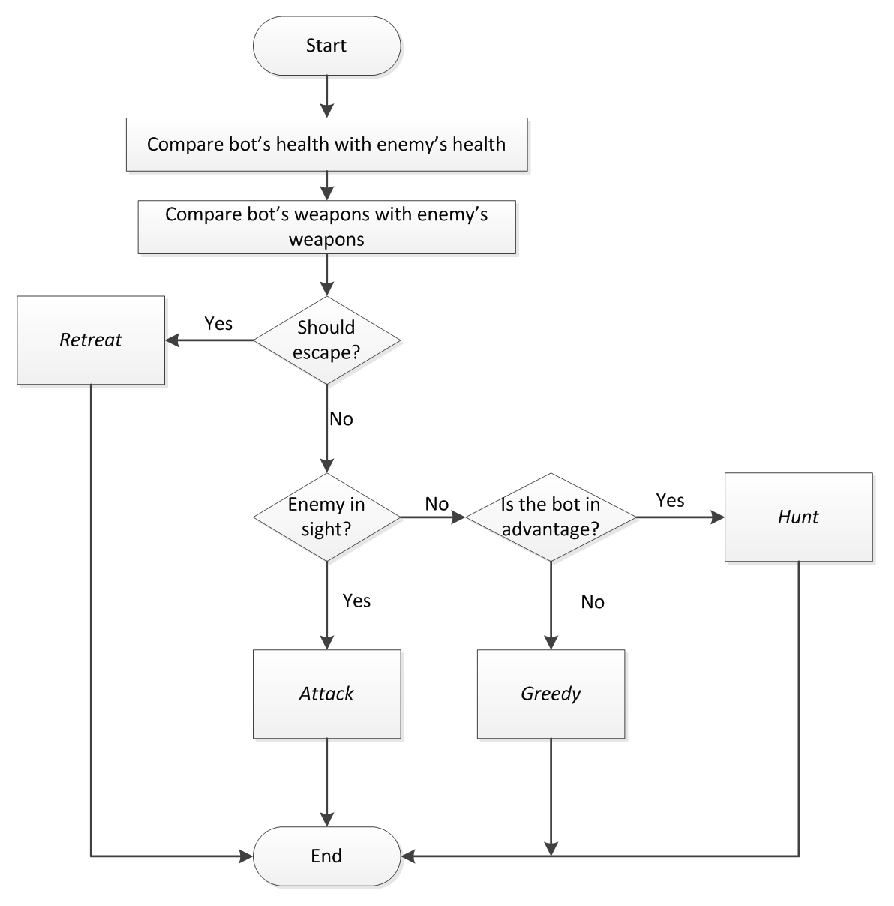
\includegraphics[scale=0.55]{imags/primary_states_flowchart.eps}
   \caption{Primary States selection flow chart}
   \label{fig:primary_states_flowchart}
\end{figure}
%
The \textit{Camp} state is not included because it is a special state with very particular conditions.
The comparisons and decisions required to choose the state are quite complex, because they consider several factors and situations that the human expert knows. For instance, the comparison between weapons depends on several parameters and weights, because of the existent balance between the power and usefulness of all of them, which could mean that a weapon is the best in a specific situation (different levels, hidden opponent, close or far enemy), but it could be the worse on a different position. 

The AI engine (composed by a huge system of rules) chooses the primary state at a  time, but while the bot is performing the actions associated to it, the engine continues checking conditions (for instance the timing of every item), receiving sensory information, or checking the bot status, for instance. This way, a secondary state can also be set. However the engine can stop and change, at any time, both the primary and/or the secondary state, depending on the conditions, received information and status, giving an extra `flexibility' level which a FSM usually do not offer.

As a general summary, the bot tends to be defensive if its health is lower than the enemy's, unless the latter has a critical health level, so the bot will attack him to win a frag. In similar health conditions the attitude depends on the weaponry (in comparison with the enemy's weapons). If the bot's health is good, it is quite aggressive.
However, there are several conditions and situations considered which could change the states and actions to perform. For example, the difference in height (levels).
The \textit{E-Bot} general flow chart can be seen in Figure \ref{fig:e-bot_flowchart}.
%
\begin{figure}[htb]
   \centering
   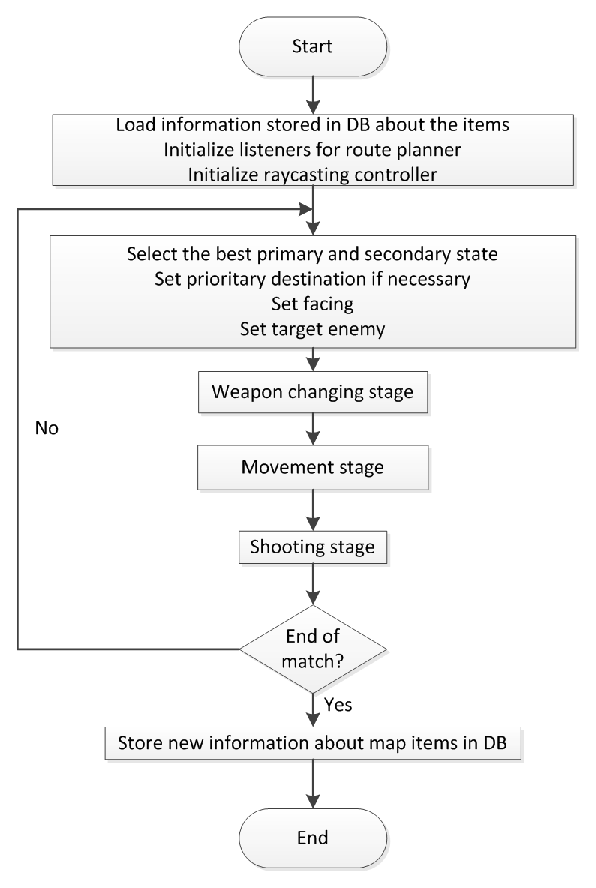
\includegraphics[scale=0.6]{imags/expert_flowchart.eps}
   \caption{\textit{E-Bot} general flow chart. The route planner controls the navigation around the map, while the raycasting controller traces vision lines for avoiding obstacles and seeing enemies.}
   \label{fig:e-bot_flowchart}
\end{figure}

%
%One bot, during a game, changes its current state depending on some factors present in its surroundings and depending on its own status and location. 
%That is, the states transitions strongly depend on a number of parameters which determine the final behaviour of the bot, since most of them are thresholds depending on which, the bot state changes (for instance, the distance to an enemy or the bot's health level). 
%These variables can be related to the individual behaviour, but some of them are also devoted to model the behaviour of the bot inside a team.
%
%In addition, the thresholds are typically compared with hard-coded values inside the source code of the bot's AI.
%This way, the state changing (and the power of the bot's AI) finally depends on some constant values.

The source code of \textit{E-Bot} is available under a GPL license at \\ {\small \texttt{https://github.com/franaisa/ExpertAgent}}.

%%%%%%%%%%%%%%%%%%%%%%%%%%%%%%   EVOLUTIONARY BOT  %%%%%%%%%%%%%%%%%%%%%%%%%%%%%

%\section{Evolution of the UT2K4 Expert Bot}
%\label{sec:evolution}
%
%Following previous approaches by us \cite{Unreal-AEB02,Mora_Unrealbot_EVO2010,Mora_UnrealTeams_CIG2010} and in the literature \cite{cole_GAtuning_cec2004}, the expert bot defined in previous section want to be optimised. To this end, is important to notice that the states transitions strongly depend on a set of parameters which act as thresholds, weights, priorities, conditions (for instance, the distance to an enemy or the bot's health level); and which finally determine the final behaviour of the bot. Thus, we can consider this set of parameters as an individual in a Genetic Algorithm (GA) \cite{GA_Goldberg89}, which can evolve their values searching for the best combination, i.e. the set of values which performs better in a battle.
%Following this idea, we have designed a GA-based bot, named \textit{GE-Bot}.
%
%On the following paragraphs we are going to describe this design.
%First, there have been defined the \textit{chromosome scheme}. It has 143 genes, grouped in different blocks, as shown in Figure \ref{fig:chromosome143}.
%
%\begin{figure}[htb]
%   \centering
%   \includegraphics[scale=0.27]{imags/chromosome143.eps}
%   \caption{\textit{GE-Bot} 143 genes chromosome}
%   \label{fig:chromosome143}
%\end{figure}
%
%As it can be seen there are six different blocks, described as follows:
%\begin{itemize}
%    \item \textit{health} (2 genes): levels to be defensive, offensive or neutral.
%    \item \textit{distance} (3 genes): close, medium and far distances for choosing a weapon to attack and/or maintain the separation with the enemy.
%    \item \textit{risk} (5 genes): number of health points that the bot could lose in an action.
%    \item \textit{time} (1 gene): time to consider an enemy as lost (from the bot point of view).
%    \item \textit{items} (6 genes): items priority for timing, i.e. which one is the most interesting for waiting its respawn.
%    \item \textit{weapon selection} (126 genes): priority of using each weapon, considering distance, height and the situation of the bot with respect to the enemy.
%\end{itemize}
%
%This chromosome length implies a high amount of generations are required for a good optimisation (as it will be commented in Section \ref{sec:experiments}), so it has been redefined just considering 26 genes. 
%
%Figure \ref{fig:chromosome26} shows the new scheme.
%
%\begin{figure}[htb]
%   \centering
%   \includegraphics[scale=0.27]{chromosome26.eps}
%   \caption{\textit{GE-Bot} 26 genes chromosome}
%   \label{fig:chromosome26}
%\end{figure}
%
%Five of the six blocks remain the same, but the weapon selection one has been reduced and redefined (just 9 genes), considering as parameters one priority associated to every weapon. Thus, the bot will consider one weapon as better than the rest in every situation.
%Of course, the behaviour obtained with this model is much simpler than with the previous scheme; however it would need much less computational effort for optimizing these parameters.
%
%The \textit{fitness function} (valuates every individual) has been defined as Equation \ref{eq:fitness}.
%
%{\footnotesize
%\begin{equation}\label{eq:fitness}
%   f =
%   \begin{cases}
%      3 + (damP/damR) & \text{if $frags + 1 = deads$}\\
%
%      (2 \cdot frags - y) + (damP/damR) & \text{if $frags > deads$}\\
%
%      (3/2) + (damP/damR) & \text{if $frags = deads$}\\
%
%      frags/deads & \text{if $frags < deads$}
%   \end{cases}
%\end{equation}
%}
%
%\begin{small}
%\begin{equation} \label{eq:fitness}
%f=\left\{ \begin{array}{ll} 
%3 + (damP/damR) & \textit{if (frags + 1) = deads}\\
%
%      (2 \cdot frags - deads) + (damP/damR) & \textit{if frags $>$ deads}\\
%
%      (3/2) + (damP/damR) & \textit{if frags = deads}\\
%
%      frags/deads & \textit{if frags $<$ deads}\\
%\end{array} \right.
%\end{equation}
%\end{small}
%
%Where $frags$ is the number of enemy kills  the bot has obtained, $deads$ is the number of own deads, $damP$ is the total damage produced by the bot, and $damR$ is the total damage it has received.
%As it can be noticed this function rewards the individuals with a positive balance (more frags than deads) and a high number of frags. In addition individuals which perform a high amount of damage to the enemies are also rewarded, even if they have not got a good balance.
%It yields a high value to remark the best individuals; meanwhile bad individuals obtain a low value.
%
%The \textit{evaluation of an individual} consists in setting the values of the chromosome in \textit{E-Bot} AI engine, conforming a \textit{GE-Bot}. Then it is launched a 1 vs 1 combat with this against the standard \textit{E-Bot}. After the time defined (usually 5 minutes), the fitness value is computed for the individual. There is a high pseudo-stochastic component in these battles, since the results do not depend completely on our bot, but also on the enemy's actions which we cannot control. Thus, the fitness function is considered as noisy \cite{Mora_noisy_Genebot_EVO2012}, since an individual could be valued as good in one combat, but yield very bad results in the next. In order to (partially) avoid this issue, some other evaluations (combats) are performed for every individual, being the final fitness value, the average of all the computations (following Equation \ref{eq:fitness}).
%
%An \textit{elitist selection mechanism} has been considered, choosing the best 4 individuals who remain in the next population. Moreover the rest of the population minus 4 is selected as parents. The 4 worse are removed.
%
%The \textit{uniform crossover} operator (every gene of a descendent has the same probability of belonging to each one of the parents) has been applied in two steps: on one hand it is used with the elite, yielding two descendents by combining the best individual with a random one in the best 4 chosen. On the other hand, the rest of the offspring is formed as a random combination of the rest of parents (in pairs). Finally, 4 random individuals are included in the population (they substitute the 4 worse) to add diversity.
%
%Finally, a \textit{mutation mechanism} is performed on every descendent. It changes with a probability equal to 1/chromosome\_size the value of every gen in a $\pm$10\%.
%
%In the case of this algorithm, and due to the high computational time it consumes the evolution (mainly for the expensive evaluation function), a database is used for storing the status in every moment (individuals, evaluations, chromosome values, etc). It lets the user to continue the execution in case of an unexpected error occurs (a machine fail, for instance), or due to a desired pause.

%The source code of both \textit{E-Bot} and \textit{GE-Bot} can be downloaded from {\small \texttt{https://github.com/franaisa/EvolutionaryBot}} under a GPL license.

%%%%%%%%%%%%%%%%%%%%%%%%%%%%%%   EXPERIMENTS  %%%%%%%%%%%%%%%%%%%%%%%%%%%%%%%

\section{\textit{E-Bot} Results}
\label{sec:experiments}
%

In order to test the expert bot some experiments has been conducted. The first consists in launching four different game matches in the \textit{1 vs 1 - Death Match} mode, having as players a game standard bot in the hardest difficulty (\textit{StdBot}), and our expert bot (\textit{E-Bot}). 

Two different arenas have been considered, namely \textit{DM-Idoma} and \textit{DM-Ironic}, since they are two of the most famous maps, used in competitions and with a design that offers almost any possible fighting situation: different levels, hidden zones, viewpoints and camping areas, etc.

The bots have been fighting following the commented championship rules (as \textit{E-Bot} was designed) along 15 minutes. The results of every match as well as the average in each map are shown in Table \ref{tab:e-bot_results}.
%
\begin{table}[htp]
\centering
\caption{Scores (number of frags) of the test fights between \textit{E-Bot} and a Standard UT2K4 bot in the hardest difficulty (\textit{StdBot}).
\label{tab:e-bot_results} }

\begin{tabular}{ccc}

\begin{tabular}{|l|r|r|}
\hline
\textit{Map} & \textit{E-Bot} & \textit{StdBot}\\
\hline
 & 17 & 6\\
\textit{DM-Ironic} & 22 & 8\\
 & 19 & 9\\
\hline
Average & 19.33 & 7.67\\
\hline
\end{tabular}

& &

\begin{tabular}{|l|r|r|}
\hline
\textit{Map} & \textit{E-Bot} & \textit{StdBot}\\
\hline
 & 23 & 14\\
\textit{DM-Idoma} & 20 & 9\\
 & 25 & 8\\
\hline
Average & 22.67 & 10.33\\
\hline
\end{tabular}

\end{tabular}
\end{table}


As it can be seen \textit{E-Bot} outperforms the standard UT2K4 bot in all the matches, even in the hardest difficulty level, which is a true challenge for a medium level human player. This leads us to conclude that the expert bot has been successfully designed and implemented.

% Subsecci�n o nueva secci�n aqu�? - JJ
% ocupar�a mucho m�s...
%The following experiments are aimed to test the value of the evolutionary approach. 
%Some tests with \textit{GE-Bot} have been performed, applying different configurations in chromosome length, number of generations, and in the evaluation function (number of matches and time of everyone).
%The parameters considered are shown in Table \ref{tab:ga-params}. Most of them have been set starting from standard GA ones, and tuning through systematic experimentation.
%
%\begin{table}[htp]
%\centering
%\caption{Parameters of GA (used in \textit{GE-Bot}).
%\label{tab:ga-params} }
%\begin{tabular}{|l|c|}
%\hline
%\textit{Number of individuals} & 30\\
%\textit{Chromosome length} & 26, 143\\
%\textit{Mutation probability} & 1/26, 1/143 \\
%\textit{Mutation rate} & $\pm$10\% \\
%\textit{Number of generations} & 30, 50 \\
%\textit{Time limit per chromosome} & 2, 3, 5 minutes \\
%\textit{Number of evaluations per chromosome} & 1, 3 \\
%\hline
%\end{tabular}
%\end{table}
% 
%Looking at the values it can be seen that the evaluation of one individual takes, depending on the configuration, from 2 to 15 minutes (3 times x 5 minutes), which means that each experiment has spend from 5 to 19 days. Since this is a preliminary study and due to the high computational cost, just one run has been performed in some experiments.
%
%It is important to notice that the \textit{opponent to evaluate every
%  individual} of \textit{GE-Bot} is always one
%\textit{E-Bot}. Moreover the map DM-Ironic, has been considered for
%all runs, because it is one of the most famous maps, used in
%competitions and with a design that offers almost any possible
%fighting situation: different levels, hidden zones, viewpoints
%and camping areas.

%---------------------------------------------------------------

%The first experiment with \textit{GE-Bot}, has performed one run with 30 generations, using the initial scheme with 143 genes per chromosome and doing 3 battles (of 5 minutes each) for evaluating every individual. The associated fitness to the individual is the average of the 3 values (each one obtained through Equation \ref{eq:fitness}). As stated, the objective of this evaluation scheme based on repetitions is trying to deal with the noisy nature of the fitness function \cite{Mora_noisy_Genebot_EVO2012}, since the results for the same individual evaluation may change from time to time, yielding good or bad values depending on the battle events and on the opponent's actions (his behaviour, and even our bot's are non-deterministic).
%
%Figure \ref{fig:GE-Bot_30-143-3t-5m} shows the best and average fitness (of the whole population) evolution in the run. 
%
%\begin{figure}[ht]
%\begin{center}
%\includegraphics[scale=0.235,angle=-90]{imags/best30gen143genes.eps}
%\includegraphics[scale=0.235,angle=-90]{imags/average30gen143genes.eps}
%\caption{Best (left) and average (right) fitness evolution in the experiment with 30 generations, 143 genes per chromosome and 3 evaluations per individual (5 minutes each). 
%\label{fig:GE-Bot_30-143-3t-5m}}
%\end{center}
%\end{figure}
% EStos dos gr�ficos o los pones juntos o los quitas. No aportan nada,
% y ocupan demasiado espacio. A qui�n se le ha ocurrido poner en
% gr�ficos diferentes el mejor y la media? - JJ
% Era por poner algo, ya que no hay resultados 'tangibles'. Si los pon�amos juntos no se ve una mielda porque se mueven en rangos distintos. Lo dejamos para la versi�n final.
%
%As it is plotted in the figure (left side), the best fitness graph proved the noise nature of the function, so even considering 3 matches for every evaluation, and having followed an elitist scheme, the best values oscillate without a clear tendency. The average results (on the right side plot) show a lightly improvement tendency, which let us think in a good (but slow) evolution and improvement of individuals (parameters) or results.
%The reasons of these light tendencies and high oscillations might be two: first the inclusion of diversity enhancement mechanisms, such as the uniform crossover or the random generation of some individuals (which substitute the four worst); the second reason could be the chromosome length, since the evolution of 143 genes might take much more generations.

%---------------------------------------------------------------

%Thus as commented in Section \ref{sec:evolution}, we decided to implement another chromosome scheme, less precise from the expert's AI performance point of view, but with a smaller and more approachable size. In addition and with the aim of reducing the computational cost, the battle time has been reduced to 2 minutes.
%So there have been considered 30 generations with 26 genes per chromosome performing 3 battles (of 2 minutes each) for evaluating every individual.
%Figure \ref{fig:GE-Bot_30-26-3t-2m} plots the graphs for the best and average fitness evolutions.
%
%\begin{figure}[ht]
%\begin{center}
%\includegraphics[scale=0.235,angle=-90]{imags/best30gen26genes.eps}
%\includegraphics[scale=0.235,angle=-90]{imags/average30gen26genes.eps}
%\caption{Best (left) and average (right) fitness evolution in the experiment with 30 generations, 26 genes per chromosome and 3 evaluations per individual (2 minutes each).
%\label{fig:GE-Bot_30-26-3t-2m}}
%\end{center}
%\end{figure}
% EStos dos gr�ficos o los pones juntos o los quitas. No aportan nada,
% y ocupan demasiado espacio - JJ
%
%As it is shown, there are again fluctuations and (very) light improving tendencies. The oscillations seem to be lighter, but what is happening is that the resulting values have been reduced (due to the shorter battle time). The average fitness tendency on the other hand is less clear this time. Thus, the reduction in the evaluation time just has meant an improvement in the computational cost (almost half of time).

%---------------------------------------------------------------

%Finally, we have tested the short chromosome scheme with a higher number of generations (50), but performing just a battle (of 5 minutes) for evaluating an individual. To better check the approach value 10 runs have been performed.
%The graphs can be seen in Figure \ref{fig:GE-Bot_50-26-5m}, where the graphs of the average values are plotted along with the standard deviation (of the 10 runs) for both the best fitness and the average fitness of the whole population.
%
%\begin{figure}[ht]
%\begin{center}
%\includegraphics[scale=0.235,angle=-90]{imags/best50gen26genes10runs.eps}
%\includegraphics[scale=0.235,angle=-90]{imags/average50gen26genes10runs.eps}
%\caption{Best (left) and average (right) fitness evolution in the experiment with 50 generations, 26 gene length and 5 minutes evaluations per individual. 10 runs.
%\label{fig:GE-Bot_50-26-5m}}
% Las desviaciones t�picas son para cuantas ejecuciones? - JJ
% lo pone 2 l�neas m�s arriba, jeje
%\end{center}
%\end{figure}
%
%Again, the graphs show fluctuations in the results, which can be also contrasted looking at the high standard deviations in both graphs. This means that the noisy nature of the fitness is not well controlled just with the repetition of battles and more `aggressive' methods should be employed. 
%The tendency in the average fitness seems to appear again as in the first experiment, and the values, that can be compared which the first (Figure \ref{fig:GE-Bot_30-143-3t-5m}) since the time for a battle is the same, are lightly better in this experiment. The reason is the smaller chromosome length, which is easier evolved (and improved).
%
%However the evolution in this scope is quite difficult, so it would be recommended the implementation of mechanisms to increase the exploitation of solutions rather than increasing diversity (as it is done here). For instance a stationary model (almost all the population is maintained from one generation to another) could be considered.

%---------------------------------------------------------------

%The last test has confronted the best individual of each \textit{GE-Bot} approach against \textit{E-Bot}, since they have been optimised for beating it (they have fought against it during the evolution).
%The average results of four matches are shown in Table \ref{tab:ge-bot_vs_e-bot_results}. They have been held in the same two maps and for 15 minutes each.
%
%\begin{table}[htp]
%\centering
%\caption{Average scores (number of frags) of the test fights between every configuration of \textit{GE-Bot} and \textit{E-Bot}. 4 battles in two maps: DM-Ironic and DM-Idoma.
%\label{tab:ge-bot_vs_e-bot_results} }
%\begin{tabular}{|l|ll|l|}
%\cline{2-3}
%\multicolumn{1}{l|}{} & \multicolumn{2}{c|}{Score} & \multicolumn{1}{l}{} \\ 
%\hline
%GE-Bot: 50gen-26chr-1ev-5min & 15.3 & 7.8 & E-Bot \\ 
%GE-Bot: 30gen-26chr-3ev-2min & 3.3 & 3.1 & E-Bot \\ 
%GE-Bot: 30gen-143chr-3ev-5min & 4.2 & 13.2 & E-Bot \\ 
%\hline
%\end{tabular}
%\end{table}
%
%The results show that \textit{GE-Bot} with a higher number of
%generations and smaller chromosome performs better than the one with
%the higher length. This result should be expected, since the
%chromosome length is a key factor in the evolution, with {\em long}
%individuals needing a high number of generations; with a similar
%number of evaluations, a smaller search space can be searched more
%efficiently. In this case, we just have performed (due to the huge
%computational time required) 30 generations for 143 genes which are
%clearly insufficient, according to the results. 
%The evolved for longer \textit{GE-Bot} (50 generations) yields a very
%good performance beating \textit{E-Bot} in average. 
%Moreover, the consideration of just one `long time' evaluation (5 minutes) performs better than three `short time' ones (2 minutes), because in the latter the individuals have not enough time to do valuable actions.
% Deber�ais decir algo de que evaluar con 5 minutos da mejores
% resultados que tres evaluaciones con dos minutos - JJ
% Hecho - Antonio

%---------------------------------------------------------------

As an additional test, our expert human player fought some matches against \textit{E-Bot}, always beating it. It is an expected result, since this player is one of the best in Spain. 
Thus, we have also proved the value of the expert bot versus four medium level human players (they play frequently but they are `non-professional'). One of them lost all the matches against the bot, and the rest had serious difficulties to beat \textit{E-Bot}, yielding a considerable amount of frags in the matches, so it could be considered as high-level enemy.


%%%%%%%%%%%%%%%%%%%%%%%%%%%%%%  CONCLUSIONS  %%%%%%%%%%%%%%%%%%%%%%%%%%%%%%%
%
\section{Conclusions and Future Work}
\label{sec:conclusions}
%

In this work, the design of a human-like bot for the First Person Shooter game Unreal Tournament\texttrademark~2004 (UT2K4) has been described. It models the expert knowledge of a Spanish high-level player so, its has been named Expert-Bot (\textit{E-Bot}). Its behaviour is shapes as a finite state machine with two levels of states (primary and secondary), each of them with an associated priority for performing actions. This work flow is flexible, so the AI engine can alter or change it depending on the conditions and on the bot's or enemy's status. Moreover, the bot uses a database for `learning' the maps, as a human player would do the first time she navigates around a new arena.
\textit{E-bot} has been designed for fighting in 1 vs 1 death match mode, considering the official competition rules.

%Then a Genetic Algorithm (GA) has been implemented to improve the parameters (thresholds, weights, priorities) that the bot's AI considers in its rule system. The evolved expert bot, named \textit{GE-Bot} has been tested considering different configurations (chromosome length, number of generations), along with an evaluation function consisting in repeated battles which are rated once they have finished, for assigning an average fitness value to every individual in the population. The aim is to deal with the noisy nature of the fitness function, since it depends on the results of the battles, which can vary for the same individual from time to time, regarding to the situation in the map or the enemy's actions which we cannot predict.

Some experiments have been conducted, firstly proving that
\textit{E-Bot} outperforms the standard UT2K4 bots, even in the
hardest difficulty level. Then, a set of matches against medium-level human players have been performed with quite good results: one human has been beaten and the rest have had high difficulties (several frags) to win.
The authors consider these results as a success, however there still remain several points of improvement to create a high competitive bot. 
According an expert player's opinion (one of the authors), \textit{E-Bot} does not perform as well as expected (from the behavioural point of view), so it would be necessary to improve its behaviour rather than its performance in results.

This way, the first line of research could be the improvement of the bot in its main flaw, the movement, since the implementation which offers Pogamut does not include jumps, which in fact are basic in an expert control. Thus, the possibility of jumping must be included in its actions, in order to model a harder opponent (more difficult to kill at least).

The database complexity could be increased for considering other important information for the bots, such as respawn points, heat zones, better paths, navigation points. But some additional work should be done in order to deal with this data in real-time, avoiding a delay in the performance of the bots. 

%The result-to-effort ratio for
%\textit{GE-Bot} is not very good, since the extremely high computation
%time that every experiment takes (from 5 to 20 days), has limited the
%number of generations and runs performed, so the improvement is not substantial. % Y las mejoras no son tan sustanciales? - JJ
% eso he puesto - Antonio
%However, the results yielded show that the best approach is that which considers a smaller chromosome size, and a higher number of generations, rather than wasting time in repeated evaluations.
%This approach has improved the results of \textit{E-Bot} and has beaten it in a set of test battles.

Once the behaviour would be improved, then several researching could be made with regard to the finite state machines improvement (set of behavioural states). Following other approaches by the authors, evolutionary computation algorithms \cite{Unreal-AEB02,Mora_Unrealbot_EVO2010} could be used to improve both, the set of behavioural rules and the set of threshold parameters which, in term, determine which rules are triggered and so, define the bot's behaviour.

Finally, another research line could be the adaptation or optimisation of \textit{E-Bot} for multiplayer and team modes, which are so far the most famous among the players.

%%%%%%%%%%%%%%%%%%%%%%%%%%%%%%   ACKNOWLEDGEMENTS %%%%%%%%%%%%%%%%%%%%%%%%%%%%%%

\section*{Acknowledgements}

This paper has been funded in part by projects P08-TIC-03903 (Andalusian Regional Government), TIN2011-28627-C04-02 (Spanish Ministry of Science and Innovation), and project 83 (CANUBE) awarded by the CEI-BioTIC UGR.
%The authors are very grateful to the Pogamut developers, specially to Michal Bida and Jakub Gemrot, by their dedication and support which has definitely aided to finish this work.


\bibliographystyle{splncs}
\bibliography{unreal_expert}

\end{document}
